\section{Australian Grand prix}

\subsection{Circuit Analysis}

\textbf{Circuit Name:} Albert Park Grand Prix Circuit (Melbourne, Australia) \\
\textbf{Length:} 5.278 km - \textbf{Laps:} 58 - \textbf{Total Distance:} 306.124 km

\begin{figure}[H]
    \centering
    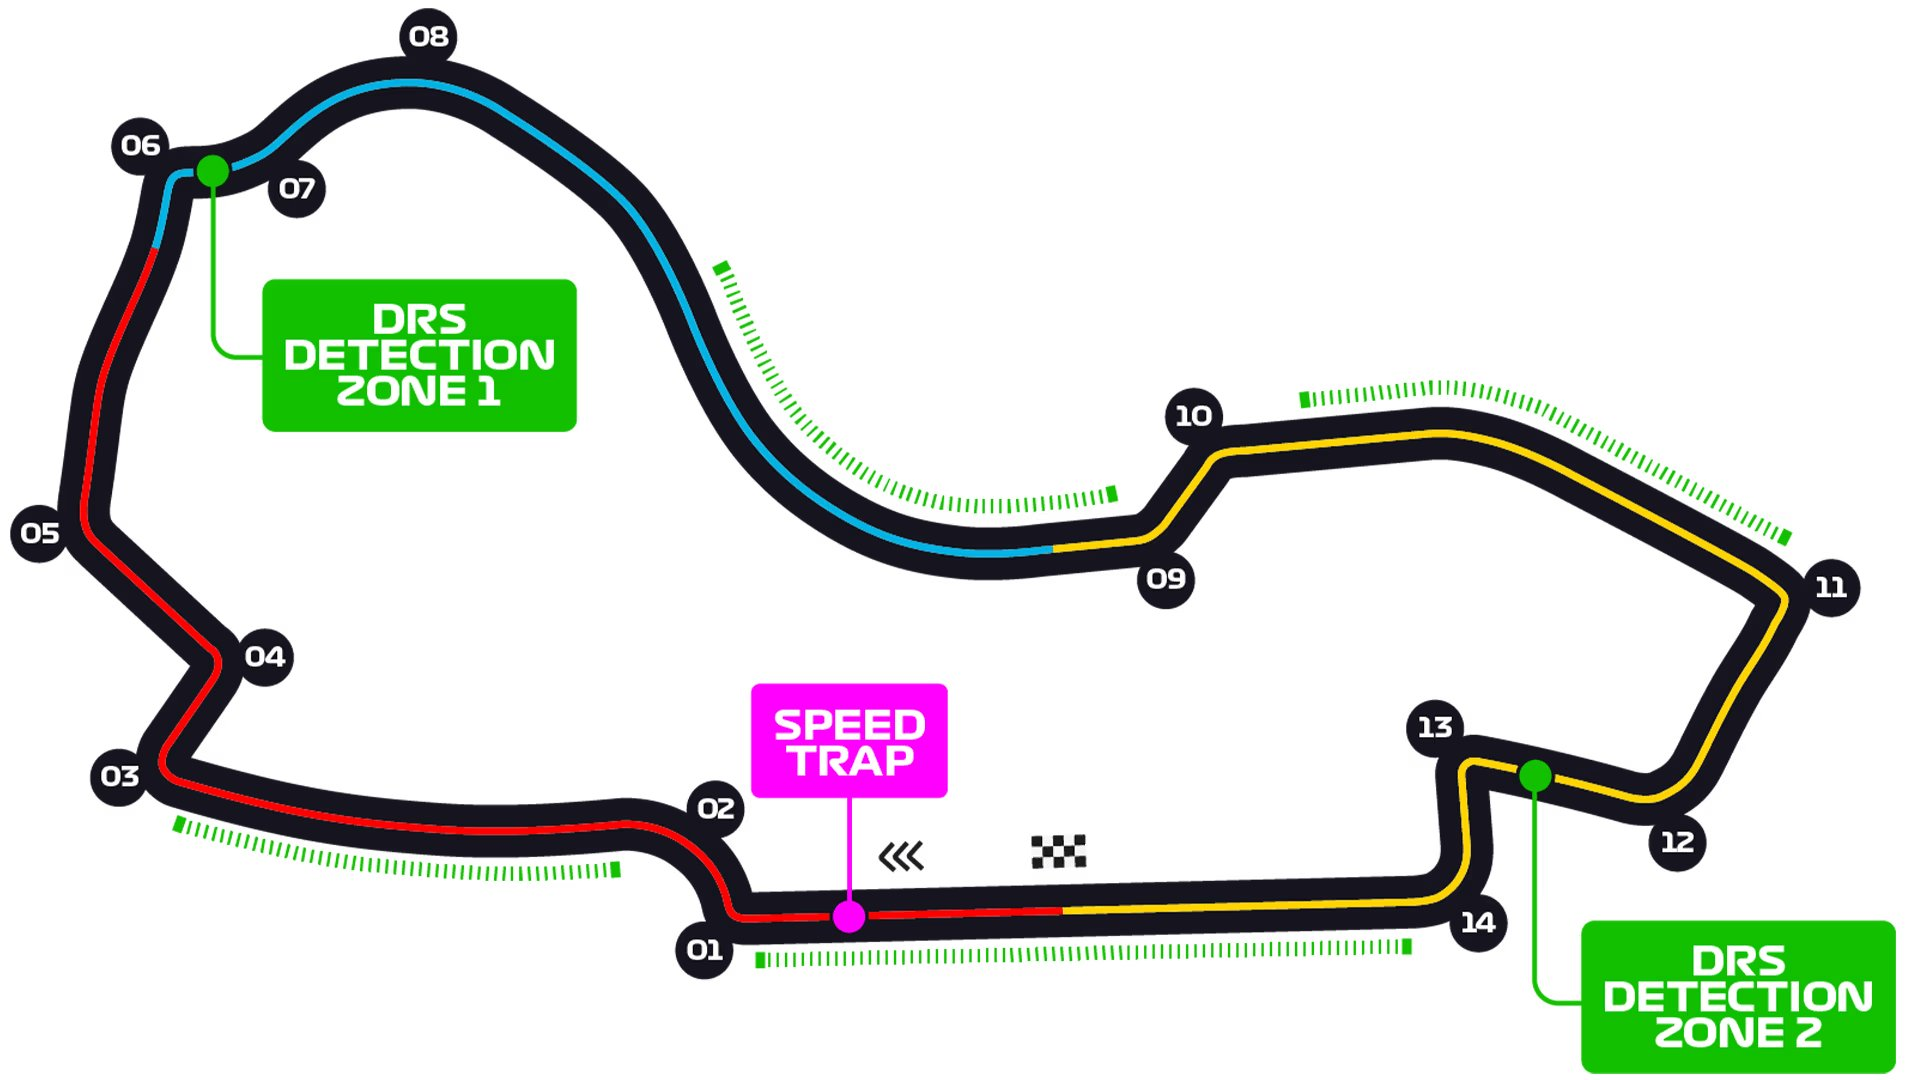
\includegraphics[width=0.75\linewidth]{images/3.Australia_Circuit.jpg}
\end{figure}

\begin{itemize}
    \item \textbf{Lap Record} : 1:16.732 (2023, Max Verstappen - Red Bull).
    
    \item \textbf{Number of Corners \& Key Features} : 16 turns (10 right, 6 left) - Tight, flowing corners.\\
    Barriers close to the track make errors costly.
    
    \item \textbf{Braking Zones \& Traction} : Several intense braking zones (e.g., Turn 1 into Turn 2 is a challenging sequence)
    
    \item \textbf{DRS \& Overtaking} : Four DRS zones: along main straight, between Turns 2 and 3, before Turn 8 and between Turns 10 and 11. \\
    Not heavy on overtaking despite having some DRS zones, primarily at Turns 1, 3, 13.
    
    \item \textbf{Tyre Degradation \& Strategy} : Tyre degradation is low, but tyre management (especially avoiding graining) is crucial.

    \item \textbf{Weather \& Environment} : Most of the time, this is a sunny weekend. Track often dusty at start of weekend.
\end{itemize}

\textbf{Strategic Summary :}
Albert Park rewards consistency, tyre preservation, and precision. Its smooth surface and moderate degradation allow varied strategies. Cars with well-balanced downforce (to handle mid-speed corners and braking) tend to do well.


\subsection{Race Analysis}

\textbf{Date:} 24 March 2024 — 15:00 local time 

\begin{itemize}
    \item \textbf{Qualifying Summary} : \textbf{Pole Position:} Max Verstappen (Red Bull) – 1:15.915 (new track record). \\
    Grid: Sainz 2nd, Norris 3rd, Leclerc 4th.\\
    Sergio Pérez, who finished 3rd during the qualifications, was penalised of three grid places for impeding.
    
    \item \textbf{Race Summary} : \textbf{Winner:} Carlos Sainz (Ferrari). \\
    \textbf{Podium:} 1. Sainz - 2. Leclerc - 3. Norris.\\
    \textbf{Technical issues:} Verstappen (brake-related mechanical failure - retired lap 3), Hamilton (engine).\\
    \textbf{Notable incidents:} Russell crashed because of Alonso (20s penalty) (Virtual Safety Car last lap).
    
    \item \textbf{Strategies} : Most runners began on medium tyres, switching to hards.\\
    - Ferrari managed tyre graining well. Sainz extended his first stint early to build a gap.\\
    - Leclerc executed a successful undercut on Norris.
    
    \item \textbf{Performance Trends} :\textbf{Ferrari} — Flawless execution: first 1–2 finish since Bahrain 2022. Sainz voted Driver of the Day. \\
    \textbf{McLaren} — Strong pace, Norris podium, Piastri close behind. \\
    \textbf{Red Bull} — Pérez distant P5, Verstappen retired early. \\
    \textbf{Mercedes} — Double DNF: Hamilton engine failure, Russell crash. First since Austria 2018.\\
    \textbf{Haas} — Double points: Hülkenberg P9, Magnussen P10. 
    
    \item \textbf{Championship Impact} : \textbf{Drivers:} Verstappen 51 points, Leclerc 47 (+1), Pérez 46 (-1).\\
    \textbf{Constructors:} Red Bull 97, Ferrari 93, McLaren 55, Mercedes 26.
\end{itemize}

\textbf{Key Takeaway :}
Ferrari capitalised on Red Bull’s misfortune and delivered a flawless strategic execution. Sainz in particular controlled tyre wear superbly, while Leclerc’s undercut secured the team valuable points.


\subsection{Link \& Takeaway}

\begin{itemize}
    \item The circuit’s low degradation meant strategic advantage went to those who conserved tyres, Ferrari mastered this, extending stints and minimising graining.
    \item The semi-street layout requires well-balanced cars for corners, Ferrari’s setup gave them the edge. McLaren and Red Bull lagged in consistent performance.
\end{itemize}